\normalfalse \difficiletrue \tdifficilefalse
\correctiontrue

%\UPSTIidClasse{11} % 11 sup, 12 spé
%\newcommand{\UPSTIidClasse}{12}

\exer{Barrière Sympact $\star\star$ \label{C1:05:14}}
\setcounter{question}{0}\marginnote{\xpComp{STAT}{03}}%\UPSTIcompetence{C1-05}
\index{Compétence C1-05}\index{Compétence STAT-03}
\index{Barrière Sympact}
\ifcorrection
\else
\marginnote{\textbf{Pas de corrigé pour cet exercice.}}
\fi

\ifprof
\else
Soit le mécanisme suivant. On a $\vect{AC}=H\vect{j_0}$ et $\vect{CB}=R\vect{i_1}$. De plus, 
$H=\SI{120}{mm}$ et $R=\SI{40}{mm}$. 

\begin{marginfigure}
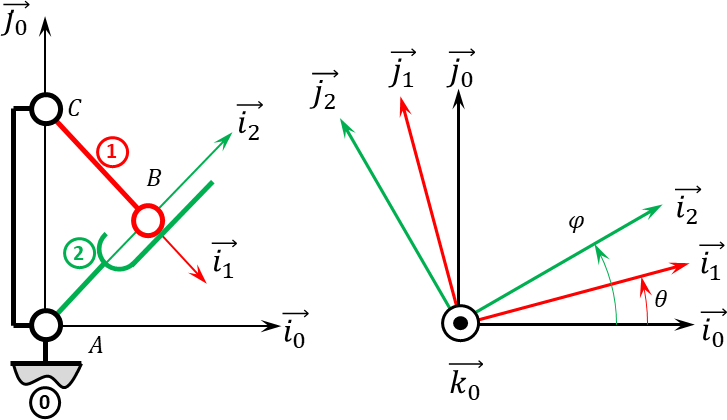
\includegraphics[width=\linewidth]{14_01}
\end{marginfigure}
\fi

On néglige la pesanteur sur la pièce \textbf{1}. 

On note $\torseurstat{F}{\text{Moteur}}{1} = \torseurl{\vect{0}}{C_m\vk{0}}{\forall P}$ l'action mécanique du moteur sur la pièce \textbf{1}.

On note $\torseurstat{F}{\text{Ressort}}{2} = \torseurl{\vect{0}}{C_r\vk{0}}{\forall P}$ l'action mécanique d'un ressort couple sur la pièce \textbf{2}. Le raideur du ressort est telle qu'il exerce un couple de \SI{45}{Nm} pour un angle de rotation 100\degres. On considère que le couple est nul lorsque la pièce 2 est à la verticale ($\varphi_0=\dfrac{\pi}{2}$). Il est au maximum lorsque $\varphi_f=0$.

On note $\torseurstat{F}{\text{Pes}}{2} = \torseurl{-Mg\vj{0}}{\vect{0}}{\forall G}$ avec $\vect{AG}=L\vi{2}$. 

\question{Réaliser un graphe d'analyse.}
\ifprof
\begin{marginfigure}
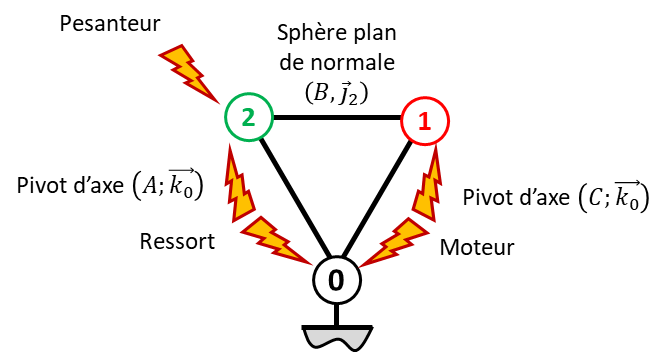
\includegraphics[width=\linewidth]{14_cor_01}
\end{marginfigure}
\else
\fi

\question{Expliciter $C_r$ en fonction des différents constantes ($k$, $\varphi_o$, $\varphi_f$) et celles qui vous sembleraient utile.}
\ifprof
Exprimons le couple du ressort par $C_r(\varphi)=a\varphi + b$. On a d'une part, $C_r(\varphi_0)=0$. D'autre part, on a une raideur $k$ de \SI{45}{Nm} pour un angle de rotation 100\degres soit $k=\dfrac{45}{100 \dfrac{\pi}{180}} = \SI{26}{Nm.rad^{-1}}$. On a donc  $C_r(\varphi_f)=k \dfrac{\pi}{2}$.

On a donc : 
$\left\{\begin{array}{l} 
a\varphi_0 + b = 0 \\
a\varphi_f + b = k \dfrac{\pi}{2}
\end{array}
\right. $
$\Leftrightarrow 
\left\{\begin{array}{l} 
 b = -a\varphi_0 \\
a\varphi_f  -a\varphi_0= k \dfrac{\pi}{2}
\end{array}
\right. $
$\Leftrightarrow 
\left\{\begin{array}{l} 
 b = -a\varphi_0 \\
a\left(\varphi_f  -\varphi_0\right)= k \dfrac{\pi}{2}
\end{array}
\right. $
$\Leftrightarrow 
\left\{\begin{array}{l} 
 b = -a\varphi_0 \\
a= k \dfrac{\pi}{2 \left(\varphi_f  -\varphi_0\right)}
\end{array}
\right. $

On a donc $C_r(\varphi)= k \dfrac{\pi}{2 \left(\varphi_f  -\varphi_0\right)}\varphi - k \dfrac{\pi \varphi_0}{2 \left(\varphi_f  -\varphi_0\right)} $.

Avec $\varphi_0=\dfrac{\pi}{2}$ et $\varphi_f=0$, on a 
%$C_r(\varphi)= -k \dfrac{\pi}{2 \dfrac{\pi}{2}}\varphi + k \dfrac{\pi \varphi_0}{2  \dfrac{\pi}{2}} $.
$C_r(\varphi)= -k \varphi + k \dfrac{\pi}{2} $.

%On a donc  $C_r(\varphi)= -k\varphi +  k \dfrac{\pi}{2}$.

%On a donc : 
%$\left\{\begin{array}{l} 
%a\varphi_0 + b = a\dfrac{\pi}{2} + b= 0 \\
%a\varphi_f + b =  b = k \dfrac{\pi}{2}
%\end{array}
%\right. $
%
%$\Leftrightarrow \left\{\begin{array}{l} 
%a= - b \dfrac{2}{\pi}= - k \dfrac{\pi}{2} \dfrac{2}{\pi} = -k \\
%b = k \dfrac{\pi}{2}
%\end{array}
%\right. $
%
%On a donc  $C_r(\varphi)= -k\varphi +  k \dfrac{\pi}{2}$
%


\else
\fi

\question{Proposer une méthode permettant d'exprimer le couple moteur en fonction des autres actions mécaniques.}
\ifprof
\begin{itemize}
\item On isole 1, on réalise un TMS en $C$ en projection sur $\vect{k_0}$. On obtient une équation liant le couple moteur et l'action normale dans la liaison sphère plan. 
\item On isole 2, on réalise un TMS en $A$ en projection sur $\vect{k_0}$. On obtient une équation liant le couple dans le ressort et l'action normale dans la liaison sphère plan. 
\item En combinant les deux équations on élimine l'action normale dans la liaison sphère plan. On peut éliminer un des deux angles en utilisant la loi entrée sortie.
\end{itemize}
\else
\fi


\ifprof
\else
\ifcolle
\else
\footnotesize
\begin{marginfigure}
\begin{tabular}{|p{.9\linewidth}|}
\hline
Indications :
\begin{enumerate}
\item .
\item $C_r(\varphi)= k \dfrac{\pi}{2 \left(\varphi_f  -\varphi_0\right)}\varphi - k \dfrac{\pi \varphi_0}{2 \left(\varphi_f  -\varphi_0\right)} $ et 
$C_r(\varphi)= -k \varphi + k \dfrac{\pi}{2} $.
\item On isole 1, TMS sur $\axe{C}{k_0}$. On isole 2, TMS sur $\axe{A}{k_0}$.
\end{enumerate} \\ \hline
\end{tabular}
\end{marginfigure}
\normalsize
\fi


\marginnote{Corrigé voir \ref{C1:05:14}.}

\fi